\section{Homotopy} 

	\begin{definition}[Homotopy]
		Let $f, g: X \to Y$ be continuous maps. $f$ is said to be \textbf{homotopic} to $g$, denoted $f \simeq g$, if there exists a continuous map $H: X \times [0, 1] \to Y$---called a \textit{homotopy}---satisfying 
		\begin{align}
			H(x, 0) & = f(x) \\ 
			H(x, 1) & = g(x) 
		\end{align}
		We claim that homotopy is an equivalence relation. 
		\begin{enumerate}
		  \item $f$ and $G$ are said to be \textbf{homotopic relative to a subset} $S \subset X$ if $H$ also satisfies 
				\begin{align}
					H(s, t) = f(s) = g(s)
				\end{align}
				for all $s \in S$. 

			\item $f$ is said to be \textbf{null-homotopic} if it is homotopic to a constant function. 
		\end{enumerate}

    \begin{figure}[H]
      \centering 
      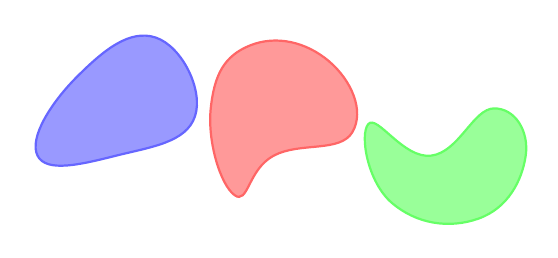
\begin{tikzpicture}
        % first blob (using random smooth cycle)
        \draw[fill=blue!40, draw=blue!60, thick] 
          plot[smooth cycle, tension=0.8] 
          coordinates {(0,0) (1,0.5) (0.5,1.5) (-0.5,1) (-1,0)};
        
        % second blob (using random smooth cycle)
        \draw[fill=red!40, draw=red!60, thick, xshift=2cm] 
          plot[smooth cycle, tension=0.8] 
          coordinates {(0,0) (1,0.3) (0.7,1.2) (-0.3,1.4) (-0.8,0.6) (-0.5,-0.5)};
        
        % third blob (using random smooth cycle)
        \draw[fill=green!40, draw=green!60, thick, xshift=4cm] 
          plot[smooth cycle, tension=0.8] 
          coordinates {(0,0) (0.8,0.6) (1.2,0) (0.6,-0.8) (-0.5,-0.6) (-0.8,0.4)};
      \end{tikzpicture}
      \caption{Think of the blobs as images of a certain function residing in $Y$. They are changing continuously. }
      \label{fig:single_homotopy_class}
    \end{figure}
	\end{definition}
	\begin{proof}
		This is clearly an equivalence relation defined on $C(X, Y)$, the set of all continuous functions from $X$ to $Y$.
		\begin{enumerate}
			\item \textit{Reflexive}. Clearly, $f$ is homotopic to itself by setting $H(x, t) = f(x)$. 

			\item \textit{Symmetric}. Given homotopy $H(x, t)$ from $f$ to $g$, the homotopy $\overline{H}(x, t) \coloneqq H(x, 1-t)$ maps from $g$ to $f$. 

			\item \textit{Transitive}. Given homotopy $H_1$ from $f$ to $g$, and homotopy $H_2$ from $g$ to $h$, the homotopy defined
				\begin{equation}
					H (x, t) \coloneqq \begin{cases}
						H_1 (x, 2t) & 0 \leq t \leq \frac{1}{2} \\
						H_2 (x, 2t - 1) & \frac{1}{2} \leq t \leq 1
					\end{cases}
				\end{equation}
				is indeed a homotopy from $F_1$ to $F_3$. To prove continuity, note that $H_1 (x, 2t)$ is continuous over the closed set $X \times [0, \frac{1}{2}]$ and $H_2 (x, 2t - 1)$ is continuous over the closed set $X \times [\frac{1}{2}, 1]$, so by the gluing lemma $H$ is continuous. 
		\end{enumerate}
	\end{proof}

	\begin{definition}[Homotopy Class]
    The space of homotopy classes from topological space $X$ to $Y$ is denoted
    \begin{equation}
      [X, Y] \coloneqq \frac{C^0 (X, Y)}{\sim}
    \end{equation}
    where $\sim$ is the homotopy relation. 
  \end{definition}

	\begin{example}[Simple Homotopy]
    If $f, g: \mathbb{R} \longrightarrow \mathbb{R}^2$ is defined as a
    \begin{equation}
      f(x) \equiv (x, x^3), \; g(x) \equiv (x, e^x)
    \end{equation}
    then the map 
    \begin{equation}
      H: \mathbb{R} \times [0,1] \longrightarrow \mathbb{R}^2, \; H(x, t) \equiv \big( x, (1-t) x^3 + t e^x \big)
    \end{equation}
    is a homotopy between them. 
  \end{example}

	\begin{example}[Another Homotopy]
    Let $id_B: B^n \longrightarrow B^n$ be the identity function on the unit $n$-disk, and let $c_0: B^n \longrightarrow B^n$ be the $0$-function sending every vector to $0$. Then, $id_B$ and $c_0$ are homotopic, with homotopy explicitly defined
    \begin{equation}
      H: B^n \times [0,1] \longrightarrow B^n, \; H(x, t) \equiv (1-t) x
    \end{equation}
  \end{example}

	The first realization is that path homotopies are trivial if the codomain is convex. 

  \begin{example}[Functions Mapping to Convex Spaces are Null-Homotopic and are Homotopic]
    If $Y = \mathbb{R}^n$, then for any space $X$, any two continuous maps $f_0, f_1: X \to \mathbb{R}^n$ are homotopic by defining the \textit{linear path homotopy}
    \begin{equation}
      F(x, t) = (1 - t) f_0 (x) + t f_1 (x) 
    \end{equation}
    which is well-defined as $Y$ is convex. Furthermore, it is path connected, and so the value of the constant function does not matter. Any two constant functions are homotopic.\footnote{Let $f, g: \mathbb{R} \longrightarrow \mathbb{R}$ be 2 continuous functions. Then $f \simeq g$, since we can construct $F: [0,1] \times \mathbb{R} \longrightarrow \mathbb{R}$ defined $F(x, t) \equiv (1-t) f(x) + t g(x)$. (Note that the set of continuous functions from $\mathbb{R}$ to $\mathbb{R}$ is a convex set.)}
  \end{example}

  \begin{example}[Two Non-Homotopic Functions]
    Consider $X = S^1, Y = \mathbb{R}^2 \setminus \{0\}$, with $f: S^1 \to Y$ the canonical inclusion, and $g$ any constant map. Then the straight line homotopy no longer works, since the circle gets ``stuck'' on the hole. That gives some sort of rigorous definition of what a hole can be. 
  \end{example}

  However, note that if two functions are null-homotopic, it \textit{does not} mean that they are homotopic to each other. 

  \begin{example}[Null-Homotopic Paths are Not Homotopic]
    Given $X = \mathbb{R}, Y = (0, 1) \cup (2, 3)$, say that we are given the functions $f, g: X \to Y$ defined $f(x) = 0.5, f(y) = 2.5$. Then by definition they are null-homotopic, but they are not homotopic to each other. 
  \end{example}

	\begin{example}[Null-Homotopic Function]
    Take a look at a function $f: \mathbb{R}^2 \longrightarrow \mathbb{R}$, which represents an arbitrary surface in $\mathbb{R}^2 \oplus \mathbb{R}$. Now, observe the constant function $c(x, y) \equiv c$, which represents a plane parallel to the $x, y$-plane. Clearly, we can imagine a deformation of the surface of $f$ to the flat surface of $c$ with the homotopy
    \begin{equation}
      H(x, t) \equiv t \, f(x) + (1-t) c(t)
    \end{equation}
    which visually represents a linear deformation of $c$ to $f$. Therefore, $f$ is null-homotopic. 
  \end{example}

  \begin{lemma}[Continuous Compositions of Homotopic Maps are Homotopic]
    Let $f_0, f_1: X \to Y$ be continuous maps with $f_0 \simeq_A f_1$. 
    \begin{enumerate}
      \item If $g: Y \to Z$ is continuous, then $g \circ f_0 \simeq_A g \circ f_1$. 
      \item If $h: W \to X$ is continuous, then $f_0 \circ h \simeq_{h^{-1}(A)} f_1 \circ h$. 
    \end{enumerate}
  \end{lemma}
  \begin{proof}
    $f_0 \simeq f_1$ implies that  there is a homotopy 
    \begin{equation}
      F: X \times [0, 1] \to Y
    \end{equation}
    s.t. $F(x, 0) = f_0 (x), F(x, 1) = f_1 (x)$. 
    \begin{enumerate}
      \item Now we construct the map 
        \begin{equation}
          G = g \circ F : X \times [0, 1] \to Z
        \end{equation}
        Then, $g$ continuous implies $G$ is continuous, and we have 
        \begin{align}
          G(x, 0) & = (g \circ F)(x, 0) = g(f_0(x)) = (g \circ f_0) (x) \\ 
          G(x, 1) & = (g \circ F)(x, 1) = g(f_1(x)) = (g \circ f_1) (x) 
        \end{align}
        which is by definition a homotopy. 
        
      \item Given $h: W \to X$ continuous, then $h \times \mathrm{id} : W \times [0, 1] \to X \times [0, 1]$ is continuous under the product topology, and so we define the continuous map 
        \begin{equation}
          H = F \circ (h \times \mathrm{id}): W \times [0, 1] \to YH
        \end{equation}
        which satisfies 
        \begin{align}
          H(x, 0) & =  (F \circ (h \times \mathrm{id})) (x, 0) = F(h(x), 0) = f_0(h(x)) = (f_0 \circ h) (x) \\ 
          H(x, 1) & =  (F \circ (h \times \mathrm{id})) (x, 1) = F(h(x), 1) = f_1(h(x)) = (f_1 \circ h) (x) 
        \end{align}
    \end{enumerate}
  \end{proof}

  Now we have seen that homotopies form an equivalence class. Now it turns out that under function compositions, homotopies are preserved, making homotopies a congruence class. 

  \begin{theorem}[Homotopies is a Congruence Relation Under Composition]
    Given $f_0, f_1: X \to Y$ and $g_0, g_1: Y \to Z$, 
    \begin{equation}
      f_0 \simeq f_1, g_0 \simeq g_1 \implies g_0 \circ f_0 \simeq g_1 \circ f_1 
    \end{equation}
  \end{theorem}
  \begin{proof}
    We have $F: [0, 1] \times X \to Y$ and $G: [0, 1] \times Y \to Z$. Then, we can simply define the component-wise composition of maps
    \begin{equation}
      G \circ (F \times \mathrm{id}): [0, 1] \times X \to Z, \qquad (G \circ (F \times \mathrm{id})) (t, x) \coloneqq G \big(t, F(t, x) \big)
    \end{equation} 
    which is continuous. Also, it is the case that 
    \begin{align}
      (G \circ F) (0, x) & = G\big(0, F(0, x) \big) = G (0, f_0 (x)) = g_0 (f_0 (x)) = (g_0 \circ f_0) (x) \\ 
      (G \circ F) (1, x) & = G\big(1, F(1, x) \big) = G (1, f_1 (x)) = g_1 (f_1 (x)) = (g_1 \circ f_1) (x) 
    \end{align}
    So this is indeed a homotopy between $g_0 \circ f_0 \simeq g_1 \circ f_1$. 
  \end{proof}

\subsection{Path Homotopies and the Fundamental Group}

	Even though we have defined what a \hyperref[pst-def:path]{path} is, let's redefine it with some other useful properties. 

	\begin{definition}[Path]
		A \textbf{path} is a continuous\footnote{We will assume the usual Euclidean subspace topology on $[0, 1]$.} map $f: [0, 1] \to X$. 
		\begin{enumerate}
			\item A \textbf{reparameterization} of a path is defined by a continuous map $\varphi: [0, 1] \to [0, 1]$ satisfying $\varphi(0) = 0, \varphi(1) = 1$. $f \circ \varphi$ is known as a \textit{reparameterized path}. 
			\item The \textbf{reverse path} of $f$ is defined as $\overline{f} (t) = f(1 - t)$. 
			\item A \textbf{loop} is a path $f$ with $f(0) = f(1) = x_0$, called a \textit{base point}. 
		\end{enumerate}
	\end{definition}
	\begin{proof}
	  A reparameterization is continuous since composition of continuous functions are continuous. The reverse is also continuous. 
	\end{proof}

  This leads to our definition of \textit{path homotopies}, which is just a specific type of homotopy. 

  \begin{definition}[Path Homotopy]
    Given two paths $f_0, f_1: [0, 1] \to X$, a \textbf{path homotopy} is a homotopy relative to $\{0, 1\}$, i.e. a continuous map $F: [0, 1] \times [0, 1] \to X$ s.t. 
    \begin{align}
      f(s, 0) & = f_0 (s) && f(s, 1) = f_1 (s) \\ 
      f(0, t) & = x && f(1, t) = x
    \end{align}
    for all $s, t$.\footnote{Note that the first line is the regular homotopy conditions, while the second line is the ``relative to''.}

		\begin{figure}[H]
			\centering 
			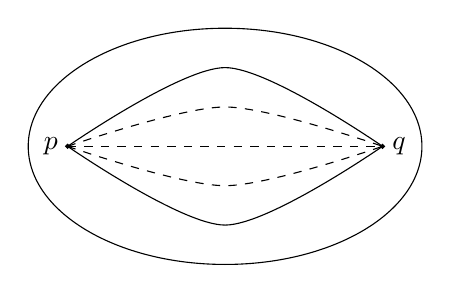
\begin{tikzpicture}[scale=0.5]
				\draw (0,0) ellipse (5 and 3); 
				\draw[fill] (-4,0) circle (0.05); 
				\draw[fill] (4,0) circle (0.05);
				\draw[dashed] (-4,0)--(4,0);
				\draw plot [smooth] coordinates{(-4,0) (0,2) (4,0)};
				\draw[dashed] plot [smooth] coordinates{(-4,0) (0,1) (4,0)};
				\draw[dashed] plot [smooth] coordinates {(-4,0) (0,-1) (4,0)};
				\draw plot [smooth] coordinates {(-4,0) (0,-2) (4,0)};
				\node[left] at (-4,0) {$p$};
				\node[right] at (4,0) {$q$};
			\end{tikzpicture}
			\caption{We can visualize two paths (sharing the same endpoints) being path homotopic if we can ``continuously deform'' one onto another.} 
			\label{fig:path_homotopy}
		\end{figure}
  \end{definition}

  \begin{corollary}[Reparameterizations are Still Path Homotopic]
    Suppose that $g: [0, 1] \to [0, 1]$ is a continuous map with $g(0) = 0, g(1) = 1$. Let $f: [0, 1] \to X$ be a path, and $f^\prime = f \circ g$. Then $f \simeq_p f^\prime$. 
  \end{corollary}
  \begin{proof}
    We can take the homotopy 
    \begin{equation}
      G: [0, 1] \times [0, 1] \to [0, 1], \qquad G(s, t) \coloneqq (1 - t) g(s) + t s 
    \end{equation}
    This is a homotopy between $g$ and the identity map $[0, 1]$ relative the endpoints since $G(s, 0) = g(s)$ and $G(s, 1) = s$. Now we compose this with $f$ to get the new continuous map  
    \begin{equation}
      F = f \circ G: [0, 1] \times [0, 1] \to X, 
    \end{equation}
    where 
    \begin{align}
      F(s, 0) & = f(G(s, 0)) = f(g(s)) = (f \circ g)(s) \\ 
      F(s, 1) & = f(G(s, 1)) = f(s) = f(s)
    \end{align} 
    and so $f \circ g \simeq_p f$. 
  \end{proof}

  The goal here is to try and develop some sort of algebraic structure on these paths. Therefore, let us define the following binary operation.  

	\begin{definition}[Composition of Paths]
		Given two paths $f, g: [0, 1] \to X$ with $f(1) = g(0)$, the composition of paths is defined 
		\begin{equation}
			f \ast g: [0, 1] \to X, \quad (f \ast g)(s) \coloneqq \begin{cases}
				f(2s) & \text{ if } 0 \leq s \leq \frac{1}{2} \\ 
				g(2s - 1) & \text{ if } \frac{1}{2} \leq s \leq 1
			\end{cases}
		\end{equation}

		\begin{figure}[H]
			\centering 
			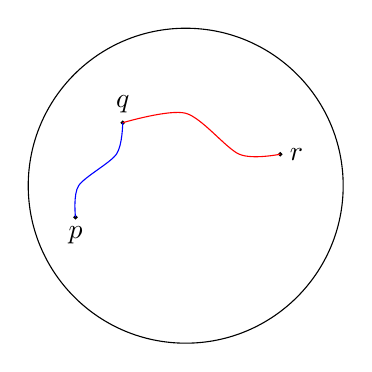
\begin{tikzpicture}[scale=0.4]
				\draw (0,0) circle (5);
				\draw[fill] (-3.5,-1) circle (0.05);
				\draw[fill] (-2,2) circle (0.05);
				\draw[fill] (3,1) circle (0.05);
				\node[above] at (-2,2) {$q$};
				\node[right] at (3,1) {$r$};
				\node[below] at (-3.5, -1) {$p$};
				\draw[blue] plot [smooth] coordinates{(-3.5,-1) (-3.4,0) (-2.2, 1) (-2,2)};
				\draw[red] plot [smooth] coordinates{(-2,2) (0,2.3) (1.7, 1) (3,1)};
			\end{tikzpicture}
			\caption{It is easy to visualize the product of two paths as the longer path created by "connecting" the two smaller paths. } 
			\label{fig:path_composition}
		\end{figure}
	\end{definition}
	\begin{proof}
		$f \ast g$ is a continuous by the \hyperref[pst-thm:pasting_lemma]{gluing lemma}.
	\end{proof}

	Note that to compose paths $f$ and $g$, we must have $f(1) = g(0)$. Therefore, path composition is a partially defined operator on the set of paths, which is a bit ugly. If we focus on the set of all \textit{loops} around $x_0$, then we can guarantee that their composition is still a loop around $x_0$. Moreover, we can upgrade this to a \textit{congruence relation}. 

	\begin{definition}[Homotopy Congruence on Loops]
	  Let $(X, x_0)$ be a pointed topological space, with loops $f, g$ about $x_0$. Then, we define the composition operation on the homotopy equivalence classes of $f$ and $g$ as
		\begin{equation}
			[f] \ast [g] \coloneqq [f \ast g]
	\end{equation}
		This turns $\simeq$ into a congruence relation. 
	\end{definition}
	\begin{proof}
	  We must show that this operation is well-defined. Let $f_0 \sim f_1$ and $g_0 \sim g_1$. Then, by definition, there exists homotopies 
		\begin{align}
			F(s, t), & \qquad F(s, 0) = f_0, F(s, 1) = f_1 \\ 
			G(s, t), & \qquad G(s, 0) = g_0, G(s, 1) = g_1 \\ 
		\end{align}
		We wish to connect the two functions $f_0 \ast g_0$ and $f_1 \ast g_1$ with a homotopy. These are just two loops anyways, so if we compose the homotopies as
		\begin{equation}
			H(s, t) \coloneqq (F_t \ast G_t) (s)
		\end{equation}
		which is a homotopy since it is continuous, with $H(s, 0) = (F_0 \ast G_0) (s) = (f_0 \ast g_0) (s)$, $H(s, 1) = (F_1 \ast G_1)(s) = (f_1 \ast g_1)(s)$, and as for the endpoints, $H(0, t) = H(1, t) = x_0$. 
	\end{proof}

\subsection{Fundamental Group}

	\begin{definition}[Fundamental Group]
		Let $(X, x_0)$ be a pointed topological space, and denote the set of congruence classes of all loops about $x_0$ as $\pi_1 (X, x_0)$. This set is an \hyperref[alg-def:group]{group} under path composition, called the \textbf{fundamental group}. 
	\end{definition}
	\begin{proof}
		We prove the group axioms. We have just proved that path composition of equivalence classes $[f] \ast [g] \coloneqq [f \ast g]$ is well-defined.
		\begin{enumerate}
			\item \textit{Closed}. Clearly, if $f, g$ are loops, then $f \ast g$ is a loop, so $[f] \ast [g] = [f \ast g]$ is a loop.
			\item \textit{Identity}. The identity element is the equivalence class of the constant map $\iota(s) = x_0$. We can see that given a path $f$, 
				\begin{equation}
				  c \ast f = \begin{cases} 
						x_0 & \text{ if } 0 \leq s \leq \frac{1}{2} \\ 
						f(2s - 1) & \text{ if } \frac{1}{2} \leq s \leq 1
					\end{cases}, \quad f \ast c = \begin{cases} 
						f(2s) & \text{ if } 0 \leq s \leq \frac{1}{2} \\ 
						x_0  & \text{ if } \frac{1}{2} \leq s \leq 1
					\end{cases}
				\end{equation}
				are reparamaterizations of $f$, so $[c \ast f] = [f \ast c] = [f]$. 

			\item \textit{Inverses}. Given $[f]$, take a representative path $f$ and take the reversed path $\overline{f}$. Then, we wish to show that $f \ast \overline{f}$ and $\overline{f} \ast f$ is homotopic to a constant path. This is a little tricky since we can't just use reparamaterizations, but let us define the homotopy from $f$ to the constant function first. 
				\begin{equation}
					f_t (s) = \begin{cases} 
						f(s) & \text{ if } 0 \leq s \leq 1 - t \\ 
						f(1 - t) & \text{ if } 1 - t \leq s \leq 1
					\end{cases}
				\end{equation}
				Then, we can define the product 
				\begin{equation}
					H_t (s) \coloneqq (f_t \ast \overline{f_t}) (s)
				\end{equation} 
				which is our desired homotopy. Therefore, $[f] \ast [\overline{f}] = [f \ast \overline{f}] = [x_0]$. 

			\item \textit{Associativity}. Given $[f], [g], [h]$, we wish to show that 
				\begin{equation}
					[f] \ast ([g] \ast [h]) = [f \ast (g \ast h)] = [(f \ast g) \ast h] = ([f] \ast [g]) \ast [h]
				\end{equation}
				Let's take representative elements $f \in [f], g \in [g], h \in [h]$. We could do this directly by defining a homotopy from $f \ast (g \ast h)$ to $(f \ast g) \ast h$, but this becomes too messy to write.\footnote{I think the actual homotopy is $F(s, t) = \begin{cases} f((t + 1) s) & \text{ if } 0 \leq s \leq \frac{1}{4} \\ g(s + \frac{t}{4}) & \text{ if } \frac{1}{4} \leq s \leq \frac{1}{2} \\ h((1 - \frac{t}{2})s + \frac{t}{2}) & \text{ if } \frac{1}{2} \leq s \leq 1 \end{cases}$.} Rather, it suffices to show that if one is a reparameterization of the other, then we are done. We can reparamaterize
				\begin{equation}
					\big( f \ast (g \ast h) \big) = \big( (f \ast g) \ast h \big) \circ \varphi, \quad \varphi(s) = \begin{cases} 
						2s & \text{ if } 0 \leq s \leq \frac{1}{4} \\ 
						s + \frac{1}{4} & \text{ if } \frac{1}{4} \leq s \leq \frac{1}{2} \\ 
						\frac{s}{2} + \frac{1}{2} & \text{ if } \frac{1}{2} \leq s \leq 1
					\end{cases}
				\end{equation}
		\end{enumerate}
	\end{proof}

  Note that the identity element of $\pi_1 (X, x_0)$ is the \textit{constant} map $x \mapsto x_0$, not the identity map! This is different from a group of transformations. We can immediately compute the fundamental group for convex sets. 

	\begin{example}[Fundamental Group of Convex Sets are Trivial]
		If $C$ is a convex set and $x \in C$, $\pi_1 (C, x) = \{e\}$, the trivial group. This is true since every loop is null-homotopic to the constant point at $x$ through a linear homotopy. 
	\end{example}

	It isn't so easy to show that a space has a nontrivial fundamental group since one must somehow demonstrate the nonexistence of homotopies between certain loops. But we can gain some intuition through some visuals. 

	\begin{example}[Visualization of the Fundamental Group of the Annulus]
		\begin{figure}[H]
			\centering 
			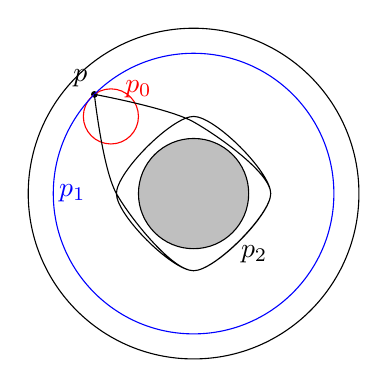
\begin{tikzpicture}[scale=0.7]
				\draw (0,0) circle (3);
				\draw[fill=lightgray] (0,0) circle (1);
				\draw[fill] (-1.8, 1.8) circle (0.05);
				\node[above left] at (-1.75, 1.75) {$p$};
				\draw[red] (-1.5, 1.4) circle (0.5);
				\node[red] at (-1, 1.9) {$p_0$};
				\node[blue] at (-2.2, 0) {$p_1$};
				\node at (1.1, -1.1) {$p_2$};
				\draw[blue] (0,0) circle (2.5455);
				\draw plot [smooth] coordinates{(-1.8, 1.8) (0, 1.3) (1.4, 0) (0, -1.4) (-1.4, 0) (0, 1.4) (1.4, 0) (0, -1.4) (-1.4, 0) (-1.8, 1.8)};
			\end{tikzpicture}
			\caption{Consider the space $X \equiv B_2 \setminus B_1$, which is the 2-disk without the unit disk in $\mathbb{R}^2$. Given an arbitrary point $p \in X$, there exists an infinite number of path classes of $X$ at $p$, denoted $[p_i]$, where $i$ corresponds to how many times the paths loop around the hole. The first three path classes are shown below. It is clear that $[p_0]$ is the identity, and the group operation rule is $[p_i] \cdot [p_j] = [p_{i+j}]$ meaning that $\pi_1(X, p)$ is the infinite discrete group generated by $[p_0]$ and $[p_1]$. } 
			\label{fig:disk}
		\end{figure}
	\end{example}

\subsection{Induced Homomorphisms}

  Now that we have constructed the fundamental group at a point $x_0$, the next things to consider are their behavior under group homomorphisms, and how different fundamental groups at different points (of the same topological space) look like. 

  \begin{definition}[Induced Group Homomorphism]
    Suppose $k: X \to Y$ is a continuous map with $x_0 \in X, y_0 = f(x_0) \in Y$. Define the map, called the \textbf{induced group homomorphism} of $k$ as 
    \begin{equation}
      k_\ast : \pi_1 (X, x_0) \to \pi_1 (Y, y_0), \qquad k_\ast ([f]) \coloneqq [k \circ f] 
    \end{equation}
    which is well defined since $f \simeq_p f^\prime$ in $X \implies k \circ f \simeq_p k \circ f^\prime$ in $Y$ as a composition with continuous functions. This is indeed a group homomorphism. 
  \end{definition}
  \begin{proof}
    Let's take a look at $f, g: [0, 1] \to X$. Then 
    \begin{equation}
      f \ast g : [0, 1] \to X, \qquad (f \ast g)(t) \coloneqq 
      \begin{cases} 
        f(2t)  & \text{ if } 0 \leq t \leq \frac{1}{2} \\ 
        g(2t - 1) & \text{ if } \frac{1}{2} \leq t \leq 1
      \end{cases}
    \end{equation}
    Therefore, mapping this through $k_\ast$ gives us 
    \begin{equation}
      k \circ (f \ast g) : [0, 1] \to Y, \qquad (k \circ (f \ast g)) (t) \coloneqq
      \begin{cases} 
        (k \circ f)(2t)  & \text{ if } 0 \leq t \leq \frac{1}{2} \\ 
        (k \circ g)(2t - 1) & \text{ if } \frac{1}{2} \leq t \leq 1
      \end{cases}
    \end{equation}
    Now take $k \circ f, k \circ g: [0, 1] \to Y$, and we can construct 
    \begin{equation}
      (k \circ f) \ast (k \circ g) : [0, 1] \to Y, \qquad \big( (k \circ f) \ast (k \circ g) \big) = \begin{cases} 
        (k \circ f) (2t) & \text{ if } 0 \leq t \leq \frac{1}{2} \\ 
        (k \circ g) (2t - 1) & \text{ if } \frac{1}{2} \leq t \leq 1
      \end{cases}
    \end{equation}
    which matches. Therefore we have $k \circ (f \ast g) = (k \circ f) \ast (k \circ g)$, and so under the congruence class 
    \begin{equation}
      k_\ast ([f] \ast [g]) = k_\ast([f \ast g]) = [k \circ f] \ast [k \circ g] = k_\ast ([f]) \ast k_\ast ([g]) 
    \end{equation}
  \end{proof}

  \begin{lemma}[Identity Map Induces Identity Group Homomorphism]
    If the continuous map between topological spaces is $k = \mathrm{id}_X$, then the induced homomorphism is simply the identity isomorphism. 
    \begin{equation}
      (\mathrm{id}_X)_\ast = (\mathrm{id}_{\pi_1 (X, x_0)}) 
    \end{equation}
  \end{lemma}
  \begin{proof}
    Just substituting with the formula above gives 
    \begin{equation}
      k_\ast ([f] \ast [g]) = [f] \ast [g] 
    \end{equation}
    and so $k_\ast$ must be the identity. 
  \end{proof}

  \begin{theorem}[Composition of Induced Group Homomorphisms]
    If $k: X \to Y$ and $l: Y \to Z$ are continuous, then 
    \begin{equation}
      (l \circ k)_\ast = l_\ast \circ k_\ast
    \end{equation}
  \end{theorem}
  \begin{proof}
    We have 
    \begin{align}
      (l \circ k)_\ast ([f]) & = [(l \circ k) \circ f ] \\ 
                             & = [l \circ  (k \circ f)] \\ 
                             & = l_\ast ([k \circ f]) \\ 
                             & = l_\ast (k_\ast ([f])) \\ 
                             & = (l_\ast \circ k_\ast) ([f]) 
    \end{align}
  \end{proof}

  \begin{corollary}[Homeomorphisms Induce Fundamental Group Isomorphisms]
    If $X \cong Y$ by a homeomorphism taking $x_0$ to $y_0$, then $\pi_1 (X, x_0) \cong \pi_1 (Y, y_0)$. 
  \end{corollary}
  \begin{proof}
    If $k: X \to Y$ is a homeomorphism, then $k: Y \to X$ is also a homeomorphism, both continuous. Then this induces the group homomorphisms $k_\ast: \pi_1 (X, x_0) \to \pi_1 (Y, y_0)$ and $k^{-1}_\ast: \pi_1 (Y, y_0) \to \pi_1 (X, x_0)$, and so from the lemma, 
    \begin{equation}
      k^{-1} \circ k = \mathrm{id}_X \implies (k^{-1} \circ k)_\ast = \mathrm{id}_{\pi_1 (X, x_0)}
    \end{equation}
		and so $(k^{-1})_\ast \circ k_\ast = \mathrm{id}_{\pi_1 (X, x_0)}$ and $k_\ast \circ (k^{-1})_\ast = \mathrm{id}_{\pi_1 (Y, y_0)}$. 
  \end{proof}

  Finally, let's talk about constructing new groups from old ones. 

  \begin{theorem}[Direct Products of Fundamental Groups]
    For any spaces $X, Y$, we have 
    \begin{equation}
      \pi_1 (X \times Y, x_0 \times y_0) \simeq \pi_1 (X, x_0) \times \pi_1 (Y, y_0)
    \end{equation}
    Moreover, the inclusion and projection maps on the topological spaces induce inclusion and projection maps on the groups. 
  \end{theorem}
  \begin{proof}
    A loop $f: I \to X \times Y$  with $f(0) = f(1) = (x_0, y_0)$ is the same as a pair of maps $f_X : I \to X$ and $f_Y : I \to Y$. A homotopy between loops is a continuous map $F: I \times I \to X \times Y$, which is the sames as a pair of homotopies $F_X$ and $F_Y$. 
  \end{proof}

  A fancy way to say this is that at every point, there is a group, and $\pi_1$ is a functor from the category of pointed topological spaces to the category of groups. 

\subsection{Simply Connected Spaces}

  Now the final thing to mention for now is that there is a group at every single point in a topological space. They may be completely different groups, but the following theorem nicely categorizes them in terms of path components. 

  \begin{theorem}[Fundamental Groups of Points in a Path Component are Isomorphic]
    If $x_0$ and $x_1$ are on the same path component of $X$, then $\pi_1 (X, x_0) \simeq \pi_1 (X, x_1)$. The actual isomorphism depends on a choice of a path from $x_0$ to $x_1$. 
  \end{theorem}
  \begin{proof}
		Let us construct a path $\gamma: [0, 1] \to X$ s.t. $\gamma(0) = x_0, \gamma(1) = x_1$. Then, let $[f] \in \pi_1 (X, x_0)$ be a loop about $x_0$. We can see that $\gamma \ast f \ast \overline{\gamma} \pi_1 (X, x_1)$ must be a loop around $x_1$. Similarly, if $[f] \in \pi_1 (X, x_1)$, then $\overline{\gamma} \ast f \ast \gamma \in \pi_1 (X, x_0)$. This establishes a bijection between $\pi_1 (X, x_0)$ and $\pi_1(X, x_1)$. It suffices to show that the map $A: [f] \mapsto [\gamma \ast f \ast \overline{\gamma}]$ is a group homomorphism. 

    Essentially, we want to start at $x_1$, go to $x_0$, loop around, and then go back to $x_1$, which is in total a loop around $x_1$. We claim that $A_h$ is an isomorphism by showing that it is a group homomorphism. 
    \begin{align}
      A_h ([f] \ast [g]) & = [\bar{h} \ast f \ast g \ast h] \\ 
                         & = [\bar{h} \ast f] \ast [g \ast h] \\ 
                         & = [\bar{h} \ast f] \ast [h \ast \bar{h}] \ast [g \ast h] \\ 
                         & = [\bar{h} \ast f \ast h] \ast [\bar{h} \ast g \ast h] \\ 
                         & = A_h ([f]) \ast A_h ([g]) 
    \end{align}
  \end{proof}

  Of course, when $x_0$ and $x_1$ are in different path components, they may or may not have isomorphic fundamental groups. Therefore, when we know a space $X$ is path connected, we can just drop the point $x_0$ and just refer to the fundamental group as $\pi_1 (X)$. 

  Therefore, if the space is path connected, the fundamental group at all points are isomorphic. But even if all the groups are isomorphic, they may be nontrivial. This motivates the following definition. 

	\begin{definition}[Simply Connected]
		A path connected topological space $X$ is \textbf{simply connected} if it meets each of the equivalent requirements. 
		\begin{enumerate}
			\item It has a trivial fundamental group.\footnote{Doesn't matter the base point, since it is path connected already.}
			\item For any two points $p, q \in X$, there is a unique homotopy class of paths connecting $p$ to $q$. 
		\end{enumerate}
  \end{definition}
	\begin{proof}
	  We prove bidirectionally. 
		\begin{enumerate}
			\item $(\rightarrow)$. Let $\gamma, \phi: [0, 1] \to X$ be two paths from $p$ to $q$. Then, $\gamma \ast \overline{\phi}$ must be null-homotopic since the fundamental group is trivial. Therefore, 
				\begin{equation}
					[\gamma] \ast [\overline{\phi}] = [\gamma \ast \overline{\phi}] = [e] = [\gamma \ast \overline{\gamma}] = [\gamma] \ast [\overline{\gamma}] 
				\end{equation}
				This implies that $[\overline{\phi}] = [\overline{\gamma}] \implies \overline{\phi} \simeq \overline{\gamma} \implies \phi \simeq \gamma \implies [\phi] = [\gamma]$. 

			\item $(\leftarrow)$. Let $f$ be a loop around $p$. We wish to show that $f$ is null-homotopic. If $f$ is constant, we are done. If not, then there exists a $q \neq p$ where $q \in \mathrm{Im}(f)$. We can then reparameterize $f$ into components 
				\begin{equation}
					f = f_1 \ast f_2, \qquad \begin{cases} 
						& f_1 (0) = p, f_1 (1) = q \\ 
						& f_2 (0) = q, f_2 (1) = p 
					\end{cases}
				\end{equation}
				Since there is a unique homotopy class, it must be the case that $[\overline{f}_1] = [f_2]$. Therefore, 
				\begin{equation}
					[f] = [f_1 \ast f_2] = [f_1] \ast [f_2] = [f_1] \ast [\overline{f}_1] = [e]
				\end{equation}
		\end{enumerate}
	\end{proof}

	Note that the actual isomorphism depends on the choice of the path $\gamma$. Note the following. 
  \begin{equation}
    \text{Simply Connected} \implies \text{Path Connected} \implies \text{Connected}
  \end{equation}

  \begin{example}[Simply Connected Spaces]
    The following are simply connected. 
    \begin{enumerate}
      \item $\mathbb{R}^n$ 
      \item Any convex subset of $\mathbb{R}^n$.
      \item Any star-shaped subset of $\mathbb{R}^n$, where a star-shaped set is defined as a set where there exists some point $x_0 \in A$ s.t. for all $y \in A$ the line segment from $x_0$ to $y$ is in $A$.  
    \end{enumerate}
  \end{example}

  \begin{theorem}[Union of Simply Connected Spaces]
    Suppose $X = U \cup V$, where $U, V$ are open and simply connected and $U \cap V$ is nonempty and path connected. Then $X$ is simply connected. 
  \end{theorem}
  \begin{proof}
    Let $x_0 \in U \cap V$. Given a loop $f$, we can factor $f$ as a composition $f = f_1 * \cdots * f_n$, where each $f_i$ is a path contained either in $U$ or in $V$, from some $x_{i-1} \in U \cap V$ to $x_i \in U \cap V$, and $x_n = x_0$. For $i = 1, \ldots, n-1$, choose a path $g_i$ from $x_0$ to $x_i$ in $U \cap V$.

    \begin{align}
      f &\simeq_p f_1 \overline{g}_1 g_1 f_2 \overline{g}_2 g_2 f_3 \ldots f_{n-1} \overline{g}_{n-1} g_{n-1} f_n\\
      &\simeq_p (f_1 \overline{g}_1)(g_1 f_2 \overline{g}_2)(g_2 f_3 \ldots f_{n-1} \overline{g}_{n-1})(g_{n-1} f_n)
    \end{align}

    Each of the factors is a loop in $U$ or $V$ based at $x_0$, so it can be contracted to $e_{x_0}$. Thus, $f \simeq e_{x_0}$, as required.
  \end{proof}

\subsection{Covering Maps}

  Now it turns out that a lot of sets are simply connected. So we will use this definition to categorize the fundamental groups of familiar spaces. However, the proofs of these requires the knowledge of covering spaces and lifts.  

  \begin{definition}[Covering Map]
    A function $p: \widetilde{X} \to X$ is a \textbf{covering map} if $p$ is
    \begin{enumerate}
      \item surjective,
      \item continuous,
      \item and for every $x \in X$ there exists an open $U \ni x$ s.t. $p^{-1} (U) = \cup_\alpha V_\alpha$, where $V_\alpha$ are open and disjoint, and $p |_{V_\alpha}: V_\alpha \to U$ is a homeomorphism.
    \end{enumerate}
    The sets $\{V_\alpha\}$ is a partition into \textbf{slices}, and $(\widetilde{X}, p)$ is said to be a \textbf{covering space} of $X$, and $X$ is said to be \textbf{evenly covered}. 

		\begin{figure}[H]
			\centering
			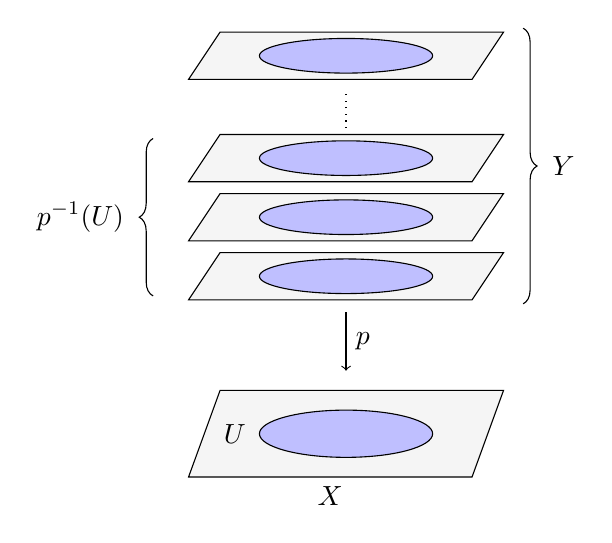
\begin{tikzpicture}[scale=1]
				% Styles
				\tikzset{
					ambient/.style={draw, fill=gray!8},
					pancake/.style={draw, fill=blue!25}
				}

				% Bottom sheet in X (parallelogram)
				\draw[ambient]
					(-1.8,-0.55) -- (1.8,-0.55) -- (2.2,0.55) -- (-1.4,0.55) -- cycle;
				\draw[pancake] (0.2,0) ellipse (1.1 and 0.3);
				\node[left] at (-0.95,0) {$U$};
				\node[below] at (0,-0.55) {$X$};

				% Map arrow
				\draw[<-] (0.2,0.8) -- (0.2,1.55);
				\node[right] at (0.2,1.18) {$p$};

				% First sheet in Y
				\draw[ambient]
					(-1.8,1.70) -- (1.8,1.70) -- (2.2,2.30) -- (-1.4,2.30) -- cycle;
				\draw[pancake] (0.2,2.00) ellipse (1.1 and 0.22);

				% Second sheet in Y (with a bit of gap above first)
				\draw[ambient]
					(-1.8,2.45) -- (1.8,2.45) -- (2.2,3.05) -- (-1.4,3.05) -- cycle;
				\draw[pancake] (0.2,2.75) ellipse (1.1 and 0.22);

				% Third sheet in Y
				\draw[ambient]
					(-1.8,3.20) -- (1.8,3.20) -- (2.2,3.80) -- (-1.4,3.80) -- cycle;
				\draw[pancake] (0.2,3.50) ellipse (1.1 and 0.22);

				% Dotted continuation upward
				\draw[dotted] (0.2,3.88) -- (0.2,4.32);

				% Another sheet above
				\draw[ambient]
					(-1.8,4.50) -- (1.8,4.50) -- (2.2,5.10) -- (-1.4,5.10) -- cycle;
				\draw[pancake] (0.2,4.80) ellipse (1.1 and 0.22);

				% Right brace for Y
				\draw[decorate, decoration={brace, mirror, amplitude=5pt}]
					(2.45,1.65) -- (2.45,5.15)
					node[midway,right=7pt] {$Y$};

				% Left brace for p^{-1}(U)
				\draw[decorate, decoration={brace, amplitude=5pt}]
					(-2.25,1.75) -- (-2.25,3.75)
					node[midway,left=7pt] {$p^{-1}(U)$};
			\end{tikzpicture}
			\caption{The best way to visualize this is to think of a ``stack of pancakes.'' Consider $Y = X \times \mathbb{Z}$ and let $p(x, z) = x$ be a projection. Given some open $U \subset X$, $p^{-1} (U) = U \times \mathbb{Z}$, with each slice $V_z = U \times \{z\}$ mapping homeomorphically onto $U$.}
			\label{fig:covering_map_pancake}
		\end{figure}
  \end{definition}

	\begin{example}[Trivial Covering Map]
		The most trivial covering map is when $\widetilde{X} = X$ and $p = \id_X$. 
	\end{example}

  \begin{example}[Covering Map of $S^1$ to Itself]
    We can consider $S^1 \subset \mathbb{C}$ and claim that the following is a covering map. 
    \begin{equation}
      p: S^1 \to S^1, \qquad p(z) = z^2
    \end{equation}
  \end{example}

	\begin{example}[Reals to the Circle]
		Given $S^1$, let us consider the covering map $p: \mathbb{R} \to S^1$ defined $p(t) = (\cos(t), \sin(t))$. It is clearly surjective and continuous. Now given any $x \in S^1$, let's take the open neighborhood $U \ni x$. Then, its preimage is the union of disjoint intervals $V_n$ for $n \in \mathbb{N}$, and if we restrict it to each $V_n$, then it is a homeomorphism. 

		\begin{figure}[H]
			\centering
			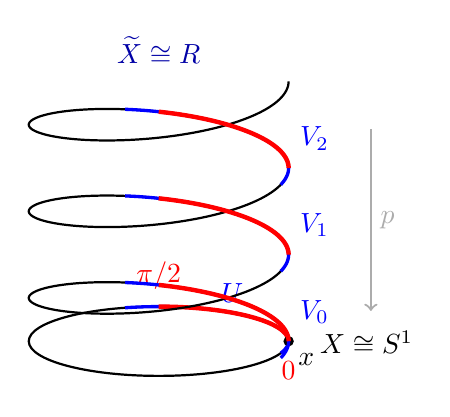
\begin{tikzpicture}[scale=1.1]
				% Colors
				\colorlet{helixblue}{blue!65!black}
				\colorlet{mapgray}{gray!65}

				% --------------------------------
				% Base space X = S^1
				% --------------------------------
				\draw[thick] (0,0) ellipse (1.5 and 0.4);

				% Label for X
				\node[black, right] at (1.75,-0.02) {$X \cong S^1$};

				% Blue open arc U on S^1
				% Chosen wide enough so the red arc [0, pi/2] lies inside it
				\draw[blue, very thick]
					({1.5*cos(-20)},{0.4*sin(-20)})
					arc[x radius=1.5, y radius=0.4, start angle=-20, end angle=105];
				\node[blue] at (0.85,0.56) {$U$};

				% Red marked arc from 0 to pi/2 on S^1
				\draw[red, ultra thick]
					({1.5*cos(0)},{0.4*sin(0)})
					arc[x radius=1.5, y radius=0.4, start angle=0, end angle=90];

				% Point x at angle 0
				\fill (1.5,0) circle (0.06);
				\node[below right] at (1.5,-0.03) {$x$};

				% Optional endpoint labels for the red arc
				\node[red, below] at (1.5,-0.12) {$0$};
				\node[red, above] at (0,0.48) {$\pi/2$};

				% --------------------------------
				% Helix = covering space
				% --------------------------------
				\draw[thick, domain=0:1080, samples=400]
					plot ({1.5*cos(\x)}, {0.4*sin(\x) + \x/360});

				% Label for covering space
				\node[helixblue] at (0,3.35) {$\widetilde{X} \cong \mathbb{R}$};

				% Blue lifts V_0, V_1, V_2 of U
				\draw[blue, very thick, domain=-20:105, samples=80]
					plot ({1.5*cos(\x)}, {0.4*sin(\x) + \x/360});
				\node[blue, right] at (1.52,0.34) {$V_0$};

				\draw[blue, very thick, domain=340:465, samples=80]
					plot ({1.5*cos(\x)}, {0.4*sin(\x) + \x/360});
				\node[blue, right] at (1.52,1.34) {$V_1$};

				\draw[blue, very thick, domain=700:825, samples=80]
					plot ({1.5*cos(\x)}, {0.4*sin(\x) + \x/360});
				\node[blue, right] at (1.52,2.34) {$V_2$};

				% Red marked lifts of the arc [0, pi/2]
				\draw[red, ultra thick, domain=0:90, samples=50]
					plot ({1.5*cos(\x)}, {0.4*sin(\x) + \x/360});

				\draw[red, ultra thick, domain=360:450, samples=50]
					plot ({1.5*cos(\x)}, {0.4*sin(\x) + \x/360});

				\draw[red, ultra thick, domain=720:810, samples=50]
					plot ({1.5*cos(\x)}, {0.4*sin(\x) + \x/360});

				% --------------------------------
				% Covering map arrow p
				% --------------------------------
				\draw[->, thick, mapgray] (2.45,2.45) -- (2.45,0.35);
				\node[mapgray, right] at (2.45,1.4) {$p$};

			\end{tikzpicture}
			\caption{The covering map $p:\widetilde{X}\to X$ visualized as a helix. The open arc $U\subset X$ has preimage
			$p^{-1}(U)=V_0\sqcup V_1\sqcup V_2\sqcup \cdots$, where each $V_\alpha$ maps homeomorphically onto $U$. The red arcs indicate the portion corresponding to angles from $0$ to $\pi/2$.}
			\label{fig:helix_covering}
		\end{figure}
	\end{example}

  \begin{example}[Positive Reals to the Circle]
    The map 
    \begin{equation}
      p: \mathbb{R}^+ \to S^1, \qquad p(x) \coloneqq ( \cos{2 \pi x}, \sin{2\pi x}) 
    \end{equation}
    is not a covering map. It is surjective and continuous but the point $x_0 = (1, 0) \in S^1$ has no neighborhood $U$ that is evenly covered by $p$. We can see that the inverse image of $(0, \epsilon)$ is not homeomorphic to an open $U$. 
  \end{example}

	Now let's introduce a few properties of covering maps.

  \begin{lemma}[Preimage of Singletons Have Discrete Topology]
    If $p: \widetilde{X} \to X$ is a covering map, then for each $x \in X$, the subspace $p^{-1} (x) \subset X$ has the discrete topology.
  \end{lemma}
  \begin{proof}
    Take some $x \in X$ and look at its preimage $p^{-1}(x)$. Then, we can imagine it as some disjoint union of discrete points, which has the discrete topology. More formally, take some open $U \ni x$ and then its preimage will be the disjoint union of open sets $\sqcup_\alpha V_\alpha$. But each point $y \in p^{-1} (x)$ will be contained in exactly one of the $U_\alpha$'s, and so $y = y \cap U_\alpha$ is open in itself, meaning that all the $\{y_\alpha\}$ will have the discrete topology. 
  \end{proof} 

  \begin{theorem}[Covering Maps are Open Maps]
    If $p: \widetilde{X} \to X$ is a covering map, then it is open, i.e. maps open sets to open sets.
  \end{theorem}
  \begin{proof}
    Suppose $A \subset \widetilde{X}$ is open. We wish to show that $p(A)$ is open. Choose an arbitrary $x \in p(A)$. By definition of covering maps, there must exist an open $U \ni x$ (but $U$ not necessarily in $p(A)$) s.t. $p^{-1} (U) = \sqcup_\alpha V_\alpha$ for $V_\alpha$ open. There is a point $y \in U$ s.t. $p(y) = x$. Let $U_\beta$ be the open slice containing $y$. Then, since $A$ is open by assumption, the set $V_\beta \cap A$ is open in $\widetilde{X}$ and hence open in $V_\beta$. Since $p$ maps $V_\beta$ homeomorphically onto $U$, it maps open sets to open sets and so $p(V_\beta \cap A)$ is open in $U$ and hence open in $X$. Furthermore, it is a neighborhood of $x$ contained in $p(A)$. Since for every $x \in p(A)$ has an open neighborhood contained in $p(A)$, $p(A)$ is thus open. 
  \end{proof}

  \begin{corollary}[Covering Maps are Quotient Maps]
    A covering map $p: \widetilde{X} \to X$ is a quotient map.
  \end{corollary}
  \begin{proof}
    This is immediate because open maps are quotient maps.\footnote{However, open doesn't mean closed!} 
  \end{proof}

  \begin{theorem}[Restriction of Covering Maps]
    Let $p: \widetilde{X} \to X$ be a covering map. If $\widetilde{X}_0 \subset \widetilde{X}$ and $X_0 = p^{-1}(\widetilde{X}_0)$, then the restriction $p_0: \widetilde{X}_0 \to X_0$ is a covering map.
  \end{theorem}
  \begin{proof}
    Given $x_0 \in X_0$, let $U \ni x_0$ be an open set. Then let $\{V_\alpha\}$ be a partition of $p^{-1} (U)$ into slices. We know that $U \cap X_0$ is an open neighborhood of $x_0$ in $X_0$, and taking the preimage we have 
    \begin{equation}
      p^{-1} (U \cap X_0) = \sqcup_\alpha V_\alpha \cap p^{-1} (X_0) = \sqcup_\alpha V_\alpha \cap \widetilde{X}_0
    \end{equation}
    The $V_\alpha \cap \widetilde{X}_0$ are disjoint, and $V_\alpha$ open in $\widetilde{X}$ implies that $V_\alpha \cap \widetilde{X}_0$ is open in $\widetilde{X}_0$. Finally, we can see that $p$ maps $V_\alpha$ homeomorphically onto $U$, and so $p$ maps $V_\alpha \cap \widetilde{X}_0$ homeomorphically onto $p(V_\alpha) \cap p(\widetilde{X}_0) = U \cap X_0$.
  \end{proof}

  \begin{theorem}[Product of Covering Maps]
    If $p: \widetilde{X} \to X$ and $p^\prime : \widetilde{X}^\prime \to X^\prime$ are covering maps, then
    \begin{equation}
      p \times p^\prime : \widetilde{X} \times \widetilde{X}^\prime \to X \times X^\prime
    \end{equation}
    is a covering map.
  \end{theorem}
  \begin{proof}
    Given $x \in X, x^\prime \in X^\prime$, let $U \ni x, U \ni x^\prime$ be open neighborhoods of $x$ and $x^\prime$ with $\{V_\alpha\}, \{V_\alpha^\prime\}$ the even slices of $p^{-1}, (p^\prime)^{-1}$. Then the preimage 
    \begin{equation}
      (p \times p^\prime)^{-1} (U \times U^\prime) = \bigcup_{\alpha, \beta} V_\alpha \times V_\beta^\prime 
    \end{equation}
    These are disjoint open sets of $\widetilde{X} \times \widetilde{X}^\prime$, each of which is mapped homeomorphically onto $U \times U^\prime$ by $p \times p^\prime$.
  \end{proof}

  \begin{theorem}[Composition of Covering Maps]
    Let $q: X \to Y$ and $r: Y \to Z$ be covering maps. If $r^{-1}(z)$ is finite for all $z \in Z$, then $p = r \circ q: X \to Z$ is a covering map. 
  \end{theorem}
  \begin{proof}
    
  \end{proof}

  What we should keep in mind is that locally, covering maps look like homeomorphisms. 

  \begin{example}[Projection of Products with Discrete Topology]
    Let $Y$ have the discrete topology, and $p: X \times Y \to X$ is a projection on the first coordinate. Then we claim that $p$ is a covering map. Note that the open sets are of the form 
    \begin{equation}
      X \times \{y\} \text{ for } y \in Y
    \end{equation}
  \end{example}

  \begin{example}
    Say $k \in \mathbb{Z} \setminus \{0\}$ and $f_k : S^1 \to S^1$ defined 
    \begin{equation}
      f_k (\cos{\theta}, \sin{\theta}) \coloneqq (\cos{k \theta}, \sin{k\theta})
    \end{equation}
    This circularly stretches out the circle by a factor of $k$. We claim that this is a covering map. 
  \end{example}

  \begin{theorem}[Covering Maps as Homeomorphisms]
    Let $p: \widetilde{X} \to X$ be a covering map with $X$ simply connected and $\widetilde{X}$ path connected. Then $p$ is a homeomorphism.
  \end{theorem}

\subsection{Lifts}
  
  There is a nice relationship between the fundamental group and the covering space. 

  \begin{definition}[Lift]
    If $p: \widetilde{X} \to X$ is a covering map and $f: Z \to X$ is continuous, then a \textbf{lift} of $f$ is a continuous map $\Tilde{f}: Z \to \widetilde{X}$ satisfying $p \circ \Tilde{f} = f$.\footnote{It is called a lift since it ``lifts'' the function with codomain $Z$ to the larger covering space $\widetilde{X}$.}

    \begin{figure}[H]
      \centering 
      \begin{tikzcd}
        & \widetilde{X} \arrow[d, "p"] \\
        Z \arrow[r, "f"] \arrow[ru, "\Tilde{f}"] & X
      \end{tikzcd}
      \caption{Commutative diagram of a lift.} 
      \label{fig:lift}
    \end{figure}
  \end{definition}

  Note that not every $f$ has a lift. However, it turns out that the existence of liftings when $p$ is a covering map is an important tool for studying covering spaces and the fundamental group. The path lifting property guarantees that paths can be lifted into a covering space. 

  \begin{lemma}[Path Lifting Property]
    Suppose $p: \widetilde{X} \to X$ is a covering map with $p(y_0) = x_0$. Given any path $f: [0, 1] \to X$ with $f(0) = x_0$, there exists a unique lift $\Tilde{f}: [0, 1] \to \widetilde{X}$ with $\Tilde{f}(0) = y_0$.
  \end{lemma}

  Therefore, this essentially means that by taking the covering map $p$ that sends $y_0$ to $x_0$ and a path $f$ starting at $x_0$, we can construct a corresponding path $\Tilde{f}$ starting at $y_0$ such that $f = p \circ \Tilde{f}$. Let's do an example. 

  \begin{example}[Lift of Real Interval to $S^1$]
    Consider the covering map and path defined as below. 
    \begin{equation}
      p: \mathbb{R} \to S^1, \qquad p(t) = (\cos{2 \pi t}, \sin{2 \pi t}) 
    \end{equation}
    We can see that $p(y_0) = p(0) = (1, 0) = x_0$. Now let's consider a few paths $f: [0, 1] \to S^1$. We would like to ``lift'' this path $I \to S^1$ to a path $I \to \mathbb{R}$. The lemma states that there is indeed a unique path. 
    \begin{enumerate}
      \item When $f(s) = (\cos{\pi s}, \sin{\pi s})$ which satisfies $f(0) = x_0 = (1, 0)$, the lift is $\Tilde{f}(t) = t/2$ which satisfies $\Tilde{f}(0) = y_0 = 0$. 
      \begin{equation}
        t \xrightarrow{\Tilde{f}} \frac{t}{2} \xrightarrow{p} \big( \cos{2 \pi \frac{t}{2}}, \sin{2 \pi \frac{t}{2}} \big) = ( \cos{\pi t}, \sin{\pi t}) = f(t)
      \end{equation}

      \item When $f(s) = (\cos{\pi s}, -\sin{\pi s})$ which satisfies $f(0) = x_0 = (1, 0)$, the lift is $\Tilde{f}(t) = -t/2$ which satisfies $\Tilde{f}(0) = y_0 = 0$. 
      \begin{equation}
        t \xrightarrow{\Tilde{f}} -\frac{t}{2} \xrightarrow{p} \big( \cos{-2 \pi \frac{t}{2}}, \sin{-2 \pi \frac{t}{2}} \big) = ( \cos{\pi t}, \sin{-\pi t}) = f(t)
      \end{equation}
      since $\cos(t) = \cos(-t)$. 
    \end{enumerate}

    \begin{figure}[H]
      \centering 
      \begin{tikzcd}
        & \mathbb{R} \arrow[d, "p"] \\
        {[a, b]} \arrow[r, "f"] \arrow[ru, "\Tilde{f}"] & S^1
      \end{tikzcd}
      \caption{} 
      \label{fig:lift_ex}
    \end{figure}
  \end{example}

  Then, we show that path homotopies can be lifted as well. 

  \begin{lemma}[Homotopy Lifting Property]
    Suppose $p: \widetilde{X} \to X$ is a covering map. If $f, g: I \to X$ are paths with $f(0) = g(0), f(1) = g(1)$, and $f \simeq_p g$ (path homotopic), and $\Tilde{f}, \Tilde{g}: I \to \widetilde{X}$ are lifts starting at the same $y_0$, then $\Tilde{f} \simeq_p \Tilde{g}$.
  \end{lemma}

  Great, so we have defined covering maps and have shown that paths admit lifts that are consistent with the path homotopy relation. Now, to connect this back to fundamental groups, we introduce the following theorem which allows us to determine the cardinality of fundamental groups through covering maps over simply connected spaces. This will be very useful to us later on.  

  \begin{theorem}[Bijection from Fundamental Group to Preimage of Covering Map on Simply Connected Space]
    If $p: \widetilde{X} \to X$ is a covering map and $\widetilde{X}$ is simply connected, then $\pi_1 (X, x_0)$ is in bijection with $p^{-1}(x_0)$.
  \end{theorem} 
  \begin{proof}
    Given a loop $f: [0, 1] \to X$ with $f(0) = f(1) = x_0$, fix $y_0 \in p^{-1} (x_0)$. By the path lifting property, we can take the lifted path $\Tilde{f}: [0, 1] \to \widetilde{X}$ with $\Tilde{f}(0) = y_0$.
    \begin{equation}
      p(\Tilde{f}(1)) = f(1) = y_0, \qquad \Tilde{f}(1) \in p^{-1} (x_0)
    \end{equation}
    By the homotopy lifting property, this only depends on $[f] \in \pi_1 (X, x_0)$. 
    \begin{enumerate}
      \item To prove surjectivity, since $\widetilde{X}$ is simply connected, this implies $\widetilde{X}$ is path connected. Choose a path $g$ from $y_0$ to $y$. Let $f = p \circ g$. Then $L([f]) = g(1) = y$.

      \item To prove injectivity, if $L ([f]) = L([g])$, then $\Tilde{f}$ and $\Tilde{g}$ are both paths in $\widetilde{X}$ from $y_0$ to $y_1$. Because $\widetilde{X}$ is simply connected, $\Tilde{f} \simeq_p \Tilde{g} \implies f \simeq_p g \implies [f] = [g]$.
    \end{enumerate}
  \end{proof}

  \begin{example}
    Take $p: \mathbb{R}^2 \to S^1 \times S^1$ defined 
    \begin{equation}
      (s, t) \mapsto \big( (\cos{2 \pi s}, \sin{2 \pi s}), (\cos{2 \pi t}, \sin{2 \pi t}) \big)
    \end{equation}
    Think back to the quotient space representation. 
    \begin{equation}
      T^2 = [0, 1]^2 /{\sim}, \qquad (x, 0) \sim (x, 1) \forall x, (0, y) \sim (1, y) \forall y
    \end{equation}
    Then we can think of $p(x, y) = (x \pmod{1}, y \pmod{1})$. We claim that this is a covering map. 
  \end{example}

\subsection{Fundamental Groups of Euclidean Space and the Sphere}

  Now that we have established that $\mathbb{R}^n$ is simply connected, along with some tools on sufficient conditions for simply connectedness and lifts, we can start to categorize fundamental groups of $\mathbb{R}^n$ and $S^n$, with the corresponding sets minus a point. 

  \begin{theorem}[Fundamental Groups of $S^n$]
    We have 
    \begin{enumerate}
      \item For $n = 1$, $S^1$ is path connected but not simply connected. 
        \begin{equation}
          \pi_1 (S^1) \simeq \mathbb{Z}
        \end{equation}

      \item For $n \geq 2$, $S^n$ is simply connected, and so 
        \begin{equation}
          \pi_1 (S^n) \simeq \{e\}
        \end{equation}
    \end{enumerate}
  \end{theorem}
  \begin{proof}
    Consider the map $p: \mathbb{R} \to S^1$ given by $t \mapsto (\cos{2 \pi t}, \sin{2 \pi t})$.\footnote{This is a classic example of what's called a covering map, which we will define later.} For each $x \in S^1$, there is an open set $U$ such that $p^{-1} (U)$ is a disjoint union of open sets $V_{i}$, where $p|_{V_i}$ is a homeomorphism. Let $x_0 = (1, 0)$. Then $p^{-1} (x_0) = \mathbb{Z}$. Then here are the key technical steps. 
    \begin{enumerate}
      \item For any continuous path $f: [0, 1] \to S^1$ with $f(0) = x_0$, and any choice of $\Tilde{x}_0 \in \mathbb{R}$ with $p(\Tilde{x_0}) = x_0$ (i.e. some integer), there is a unique continuous function $\Tilde{f}: [0, 1] \to \mathbb{R}$ with $f(0) = \Tilde{x_0}$. 
      \item $\Tilde{f}(1) - \Tilde{f}(0)$ measures the ``net winding'' of $f$. $1/2\pi$ times the net increase in the angle coordinate. In particular, if $f$ is a loop, then $\Tilde{f} (1) - \Tilde{f}(0)$ is an integer, which we'll call the \textit{winding number} of $f$, denoted $\omega (f)$. This doesn't depend on which choice of $\Tilde{f}$ we made. 
      \item Given two loops $f, g$ based at $x_0$, let $\Tilde{f}, \Tilde{g}$ by their lifts, with say $\Tilde{f}(0) = \Tilde{g}(0) = 0$. Then $f \simeq_p g$ iff $\Tilde{f} \simeq p \Tilde{g}$. One direction is easy. If $F$ is a path homotopy between $\Tilde{f}$ and $\Tilde{g}$, then $p \circ F$ is a path homotopy between $f$ and $g$. The other direction requires a somewhat elaborate argument using compactness. 
      \item As a consequence, we see that if $f \simeq_p g$, then $\Tilde{f} (1) = \Tilde{g} (1)$, and hence $\omega (f) = \omega(g)$. 
      \item Conversely, if $\omega(f) = \omega(g) = n$, then $\Tilde{f}$ and $\Tilde{g}$ are both paths in $\mathbb{R}$ from $0$ to $n$. There is a straight line homotopy between them. $F(s, t) = (1 - t) \Tilde{f} (s) + t \Tilde{g}(s)$. So $f \simeq_p g$. 
      \item We then have $\omega(f \ast g) = \omega(f) + \omega(g)$. 
      \item Thus, the winding number gives us an isomorphism from $\pi_1 (S^1) \to \mathbb{Z}$. 
    \end{enumerate}
    By using the function $p: \mathbb{R}_+ \times \mathbb{R} \to \mathbb{R}^2 \setminus \{0\}$, given by $p(r, t) = (r \cos{2 \pi t}, r \sin{2 \pi t})$, we can use the same logic. Another way to see it is that $\mathbb{R}^2 \setminus \{0\} \cong S^1 \times (0, \infty) \cong S^1 \times \mathbb{R}$. 
  \end{proof}

  Now we explore the fundamental groups of $S^n$ minus a point. This becomes very simple once we know the stereographic projection. 

  \begin{theorem}[Stereographic Projection]
    We claim 
    \begin{equation}
      S^n \setminus \{n\} \cong \mathbb{R}^{n}
    \end{equation}
  \end{theorem}
  \begin{proof}
    We can construct a formula, but visually, we can take any $x \in S^n \setminus \{n\}$, and there is a unique line $L$ through $x$ and $n$. Now let $f(x) \coloneqq L _x \cap (\mathbb{R}^{n-1} \times \{0\})$, which is bijective. It also turns out to be a homeomorphism. 
  \end{proof}

  \begin{corollary}[Fundamental Groups of $S^n$ Minus a Point]
    We claim that $S^n \setminus \{p\}$ is simply connected, for all $n \in \mathbb{N}$. 
    \begin{equation}
      \pi_1 (S^n) \simeq \{e\}
    \end{equation}
  \end{corollary}

  So informally, $S^n$ minus a point gives us $\mathbb{R}^n$, so what if we remove a point from $\mathbb{R}^n$? It turns out that by taking $n$ points away from $S^n$, it is equal to taking $n-1$ points away from $\mathbb{R}^n$. 

  \begin{theorem}[Fundamental Groups of $\mathbb{R}^n$ Minus a Point]
    We claim that 
    \begin{enumerate}
      \item For $n = 1$, $\mathbb{R} \setminus \{0\}$ is not even path connected. For any $x_0$, we have 
        \begin{equation}
          \pi_1 (\mathbb{R} \setminus \{0\}) \simeq \{e\}
        \end{equation}

      \item For $n = 2$, $\mathbb{R}^2 \setminus \{0\}$ is path connected, but it is not simply connected.\footnote{We can think of this as a hole in the middle of the plane that paths cannot unwind through.}
        \begin{equation}
          \pi_1(\mathbb{R}^2 \setminus \{x\}) \simeq \mathbb{Z}
        \end{equation}

      \item For $n \geq 3$, $\mathbb{R}^n \setminus \{x\}$ is simply connected.\footnote{We can interpret as if the extra dimensions being added gives more space for a path to unwind.}
    \end{enumerate}
  \end{theorem}
  \begin{proof}
    For $n = 1$, we can see that $(-\infty, 0)$ and $(0, +\infty)$ are convex subsets, so they are simply connected. For $n = 2$, we can see in polar coordinates, 
    \begin{equation}
      \mathbb{R}^2 \setminus \{0\} \simeq S^1 \times (0, +\infty) \implies \pi_1 (\mathbb{R}^2 \setminus \{0\}) \simeq \pi_1 (S^1) \times \pi_1 ((0, +\infty)) \simeq \mathbb{Z} \times \{e\} \simeq \mathbb{Z}
    \end{equation}
    For $n = 3$, we can construct it from smaller simply connected spaces. Take 
    \begin{align}
      U & = \mathbb{R}^n \setminus \{(0, \ldots, 0, z) \mid z \geq 0\} \\
      V & = \mathbb{R}^n \setminus \{(0, \ldots, 0, z) \mid z \leq 0\}
    \end{align}
    These are each open (since the axes that we minus out is closed) and simply connected (since they are star convex). Also, $U \cap V = (\mathbb{R}^{n-1} \setminus \{0\}) \times \mathbb{R}$, which is path connected since we assumed that $n \geq 3$. Therefore, by the theorem above, $\mathbb{R}^n \setminus \{0\}$ is simply connected. 
  \end{proof}

  \begin{theorem}[Fundamental Groups of $\mathbb{RP}^n$]
    We claim that. 
    \begin{enumerate}
      \item For $n = 1$, $\mathbb{RP}^1 \cong S^1$ and so $\pi_1(\mathbb{RP}) \simeq \mathbb{Z}$. 
      \item For $n \geq 2$, $\pi_1 (\mathbb{RP}^n) \simeq \mathbb{Z}_2$
    \end{enumerate}
  \end{theorem}
  \begin{proof}
    For $n = 1$, recall that $S^1$ is homeomorphic to $S^1/{\sim}$ where $x \sim -x$ through the homeomorhism $z \mapsto z^2$. 

    For $n \geq 2$, we claim that the projection map $p: S^n \to \mathbb{RP}^n$ defined $-\pm x \to x$ is a covering map. Furthermore, we know that $S^n$ is simply connected (since it's homeomorphic to $\mathbb{R}^n \setminus \{0\}$), and therefore there exists a bijection from $\pi(\mathbb{RP}^n, x_0)$ with $p^{-1} (x_0) = \{\pm x_0\}$. Therefore the order of the fundamental group must be $2$, and it can only be $\mathbb{Z}_2$ for all $x_0$. 
  \end{proof}

  At this point it's pretty easy to show the fundamental groups of familiar quotient spaces. 

  \begin{example}[Torus]
    The torus $T \cong S^1 \times S^1$ is path connected has the fundamental group 
    \begin{equation}
      \pi_1 (T) \simeq \pi_1 (S^1) \times \pi_1 (S^1) \simeq \mathbb{Z} \times \mathbb{Z}
    \end{equation}
    So it is not simply connected. 
  \end{example}

  \begin{example}[Cylinder]
    The cylinder is path connected and the fundamental group is 
    \begin{equation}
      \pi_1 (S^1 \times [0, 1]) \simeq \pi_1 (S^1) \times \pi_1 ([0, 1]) \simeq \mathbb{Z} \times \{e\} \simeq \mathbb{Z} 
    \end{equation}
  \end{example}

  \begin{example}[Mobius Strip]
    The Mobius strip is not simply connected. 
  \end{example}

  \begin{example}[Klein Bottle]
    The Klein bottle is not simply connected and it is not abelian. 
  \end{example}

\subsection{Retractions}

  \begin{definition}[Retraction]
    If $A \subset X$, a retraction $r: X \to A$ is a continuous function such that $r(a) = a$ for all $a \in A$.  
  \end{definition}

  \begin{example}
    The following are retractions. 
    \begin{equation}
      r: \mathbb{R} \to \{x\} \subset \mathbb{R}, \qquad r(x) = x
    \end{equation}
    This is also a retraction. 
    \begin{equation}
      r: \mathbb{R} \setminus \{0\} \to S^{n-1}, \qquad x \mapsto \frac{x}{\|x\|} 
    \end{equation}
  \end{example}

  \begin{lemma}[Group Homomorphism Induced By Retraction]
    Given $A \subset X$, a retraction $r: X \to A$, and the canonical injection $\iota: A \to X$, 
    \begin{enumerate}
      \item The induced homomorphism $r_\ast: \pi_1 (X, a_0) \to \pi_1 (A, a_0)$ is surjective. 
      \item The induced homomorphism $\iota_\ast: \pi_1 (A, a_0) \to \pi_1 (X, a_0)$ is injective. 
    \end{enumerate}
  \end{lemma}
  \begin{proof}
    
  \end{proof}

  It's pretty easy to show whether a particular example is a retraction or not. However, we will mainly be interested in the existence of retractions. 

  \begin{theorem}[Unit Interval to Endpoints]
    There is no retraction from $D^1 = [-1, 1]$ to $S^0 = \{-1, 1\}$. 
  \end{theorem}
  \begin{proof}
    Let $X = [a, b]$. There is no retraction $f: X \to \{a, b\}$ since $\im(f)$ must be connected. But $f(a) = a, f(b) = b$. Alternatively, we can use IVT. 
  \end{proof}

  \begin{theorem}[Unit Disk to Circular Boundary]
    There is no retraction from $D^2 \to S^1$. Intuitively, we can see that the mapping has to ``tear'' the disk somewhere!
  \end{theorem}
  \begin{proof}
    
  \end{proof}

  \begin{theorem}
    Let $A \subset X$, and $x_0 \in A$, and $r: X \to A$ be a retraction. Then the induced map $r_\ast: \pi_1 (X, x_0) \to \pi_1 (A, x_0)$ is surjective. 
  \end{theorem}
  \begin{proof}
    Given retraction $r: X \to A$ and the canonical injection $\iota: A \to X$, we have $r \circ \iota = \mathrm{id}_A$ by definition. Now see how it affects the fundamental spaces. 
    \begin{equation}
      \pi_1 (A, x_0) \xrightarrow{\iota_\ast} \pi_1 (X, x_0) \xrightarrow{r_\ast} \pi_1 (A, x_0)
    \end{equation}
    Therefore $r_\ast \circ \iota_\ast = \mathrm{id}_A$. So for any loop $[f] \in \pi_1 (A)$, $[f] = r_\ast (i_\ast ([f]))$, so $[f] \in \im(r_\ast)$. Also $\iota_\ast$ is injective. 
  \end{proof}

  \begin{corollary}
    If $X$ is simply connected and $A$ is not, then there is no retraction. 
  \end{corollary}

  Extending this a bit, remember that any continuous function $f: [a, b] \to [a, b]$ must have a fixed point by IVT. Thinking $D^1 = [-1, 1]$, we claim the following. Note that a rotation of the disk $D^2$ has a fixed point in the center. 

  \begin{theorem}[Brower's Fixed Point Theorem]
    Any continuous function $f: D^2 \to D^2$ has a fixed point, i.e. there exists $x \in D^2$ s.t. $f(x) = x$.\footnote{This was first proven in the 1930s based on a non-intersection theorem . But it is non-constructive, i.e. doesn't show you how to find the point. }
  \end{theorem}
  \begin{proof}
    Suppose $f: D^2 \to D^2$ has no fixed point. Define a function $g: D^2 \to D^2$ as follows. For $x$, take $f(x) \neq x$ and draw a ray from $f(x)$ to $x$ (directions matter!). Where it hits the boundary is the output $g(x)$. It is much more tedious to write out in formulas, but if you do, you can see that it's just the composition of continuous functions and is so continuous. If $x \in S^1$, then $g(x) = x$, so I've just constructed a retraction from $D^2$ to $S^1$, which is a contradiction! 
  \end{proof}

  So what about higher dimensions? If we believe that there is no retraction $D^n \to S^{n-1}$, by the same method we can prove for $D^n \to D^n$. The problem is that for $n \geq 2$ $S^{n-1}$ is simply connected and so $\pi_1(S^{n-1}) = \{e\}$, and same holds for $D^n$. So we can't prove the non-retraction using fundamental groups $\pi_1$. This is where we need higher order homotopy groups. 

\subsection{Exercises}

  \begin{exercise}[Munkres 51.1]
    Show that if $h, h' : X \to Y$ are homotopic and $k, k' : Y \to Z$ are homotopic, then $k \circ h \text{ and } k' \circ h'$ are homotopic.
  \end{exercise}
  \begin{solution}
    From the assumptions there exists homotopies $H: X \times I \rightarrow Y$ and $K: Y \times I \rightarrow Z$. We define the composition homotopy as 
    \begin{equation}
      G: X \times I \rightarrow Z, \qquad G(x, t) \coloneqq K(H(x, t), t)
    \end{equation}
    Note that since $(x, t) \mapsto H(x, t)$ is continuous, by the product topology the map $(x, t) \mapsto (H(x, t), t)$ is continuous, and it composed with continuous $K$ makes it also continuous. Finally, we have 
    \begin{align}
      G(x, 0) & = K(H(x, 0), 0) = K(h(x), 0) = k(h(x)) = (k \circ h) (x) \\ 
      G(x, 1) & = K(H(x, 1), 1) = K(h^\prime (x), 1) = k^\prime (h^\prime (x), 1) = (k^\prime \circ h^\prime) (x)
    \end{align}
  \end{solution}

  \begin{exercise}[Munkres 51.2]
    Given spaces $X$ and $Y$, let $[X, Y]$ denote the set of homotopy classes of maps of $X$ into $Y$.
    \begin{enumerate}
      \item[(a)] Let $I = [0, 1]$. Show that for any $X$, the set $[X, I]$ has a single element.
      \item[(b)] Show that if $Y$ is path connected, the set $[I, Y]$ has a single element.
    \end{enumerate}
  \end{exercise}
  \begin{solution}
    Listed. 
    \begin{enumerate}
      \item Take continuous $f, g: X \rightarrow I$ and define the homotopy $F: X \times I \rightarrow I$ between them as the convex combination 
      \begin{equation}
        F(x, t) = (1 - t) f(x) + t g(x)
      \end{equation}
      We have $F(x, 0) = f(x)$ and $F(x, 1) = g(x)$, and the products/sums of continuous maps are continuous. Finally, we can see that $F(x, t) \in I$ because given any $x$, 
      \begin{align}
        f(x) \leq g(x) & \implies f(x) \leq F(x, t) = (1 - t) f(x) + t g(x) \leq g(x) \\
        f(x) \geq g(x) & \implies g(x) \leq F(x, t) = (1 - t) f(x) + t g(x) \leq f(x)
      \end{align} 
      for all $t \in [0, 1]$, and since $[0, 1] \subset \mathbb{R}$ is convex, $F(x, t) \in [0, 1]$ for all $t$ and $x$. 

      \item Given any continuous function $f: I \rightarrow Y$, this is by definition a path. We wish to show that this is homotopic to a constant map, say the value at $f(0) \in Y$. We construct the homotopy 
      \begin{equation}
        F(x, t): I \times I \rightarrow Y, \qquad F(x, t) = f((1 - t) x)
      \end{equation}
      This satisfies $F(x, 0) = f(x)$ and $F(x, 1) = f(0)$. This is also continuous since it is the composition of continuous $(x, t) \mapsto (1 - t)x$ and continuous $f$. Therefore, given two functions $f, g: I \rightarrow Y$, we know that $f \simeq f(0)$ and $g \simeq g(0)$. Now since homotopy is an equivalence relation, it suffices to show that $f(0) \simeq g(0)$, i.e. any two constant functions are homotopic. Since $Y$ is path connected, there exists a path $h: I \rightarrow Y$ such that $h(0) = f(0), h(1) = g(0)$. Now we define the homotopy 
      \begin{equation}
        H: I \times I \rightarrow Y, \qquad H(x, t) = h(t)
      \end{equation}
      which is certainly continuous since path $h$ is continuous by definition, and $h(0) = f(0), h(1) = g(0)$. 
    \end{enumerate}
  \end{solution}

  \begin{exercise}[Munkres 51.3]
    A space $X$ is said to be \textit{contractible} if the identity map $i_X : X \to X$ is nullhomotopic.
    \begin{enumerate}
      \item[(a)] Show that $I$ and $\mathbb{R}$ are contractible.
      \item[(b)] Show that a contractible space is path connected.
      \item[(c)] Show that if $Y$ is contractible, then for any $X$, the set $[X, Y]$ has a single element.
      \item[(d)] Show that if $X$ is contractible and $Y$ is path connected, then $[X, Y]$ has a single element.
    \end{enumerate}
  \end{exercise}
  \begin{solution}
    Listed. 
    \begin{enumerate}
      \item For $I$, we define the homotopy $F(x, t) = (1 - t)x$, which is continuous (since it is a scalar multiple of the continuous identity map) and satisfies $F(x, 0) = x = i_X(x)$, and $F(x, 1) = 0$ which is a constant map. For $\mathbb{R}$ we can use the same homotopy and the same logic follows. 

      \item Given that $X$ is nullhomotopic let $z \in X$ be the value of the constant map that is homotopic to the identity $i: X \rightarrow X$, with homotopy $F: X \times I \rightarrow X$ where $F(x, 0) = x$ and $F(x, 1) = z$. Then we claim that for any $x \in X$, $x$ is path connected to $z$ since by fixing $x$, the function $\gamma: I \rightarrow X$ defined $\gamma(t) = F(x, t)$ is a path: it is continuous, $\gamma(0) = F(x, 0) = x$, and $\gamma(1) = F(x, 1) = z$. Therefore we have found such a path, and since path connectedness is an equivalence relation, for any $x, y \in X$, $x \sim z \sim y$, making $X$ path connected. 

      \item Since $Y$ is contractible, let us construct the homotopy of the constant map to the identity map $F: Y \times I \rightarrow Y$ satisfying $F(y, 0) = z$ for some $z \in Y$ and $F(y, 1) = y$. Now given continuous $g: X \rightarrow Y$, we wish to show that it is homotopic to the constant map with value $z$. Consider the homotopy $G: X \times I \rightarrow Y$ defined 
      \begin{equation}
        G(x, t) = F(g(x), t)
      \end{equation}
      This is clearly continuous as the composition of continuous maps. Furthermore, $G(x, 0) = F(g(x), 0) = z$ and $G(x, 1) = F(g(x), 1) = g(x)$, making this indeed a homotopy. Since homotopy is an equivalence relation for any continuous $f, g: X \rightarrow Y$, $f \simeq z \simeq g$, and so there is only one equivalence class. 

      \item We wish to show that given any two functions $f, g: X \rightarrow Y$, $f \simeq g$. Since $X$ is contractible, there exists a homotopy $F: X \times I \rightarrow X$ where $F(x, 0) = z$ for some $z \in X$ and $F(x, 1) = x$. We can take $f, g$ and see that $(f \circ F), (g \circ F): X \times I \rightarrow Y$ is a homotopy, as the composition of continuous maps satisfying 
      \begin{align}
        (f \circ F)(x, 0) & = f(F(x, 0)) = f(z) \\ 
        (f \circ F)(x, 1) & = f(F(x, 1)) = f(x) \\ 
        (g \circ F)(x, 0) & = g(F(x, 0)) = g(z) \\ 
        (g \circ F)(x, 1) & = g(F(x, 1)) = g(x) 
      \end{align}
      Therefore, $f(z) \sim f$ and $g(z) \sim g$. We know that since $Y$ is path connected, $f(z) \sim g(z)$ as given in my argument in Munkres 51.2.b, and so $f \sim f(z) \sim g(z) \sim g$, and every continuous function is a part of the same equivalence class. 
    \end{enumerate}
  \end{solution}




\section{Other}

  We can also expect that since homotopy is clearly a topological property, it is preserved under continuous maps. We state this result formally in the following lemma.

  \begin{lemma}
    If $F_0, F_1: X \longrightarrow Y$ and $G_0, G_1: Y \longrightarrow Z$ are continuous maps such that $F_0 \simeq F_1$ and $G_0 \simeq G_1$, then 
    \[G_0 \circ F_0 \simeq G_1 \circ F_1\]
    Similarly, if $f_0, f_1: I \longrightarrow X$ are path homotopic, and $F: X \longrightarrow Y$ is a continuous map, then 
    \[F \circ f_0 \sim F \circ f_1\]
    Thus, if $F: X \longrightarrow Y$ is a continuous maps, for each $q \in X$, we can construct a well-defined map
    \[F_*: \pi_1 (X, q) \longrightarrow \pi_1 \big( Y, F(q)\big)\]
    by setting
    \[F_* ([f]) \equiv [F \circ f]\]
  \end{lemma}

  \begin{lemma}
    If $F: X \longrightarrow Y$ is a contiuous map, then the induced map 
    \[F_* : \pi_1(X, q) \longrightarrow \pi_1 \big( Y, F(q)\big)\]
    is a group homomorphism. 
    \begin{tikzpicture}
        \node at (0,0) {x};
    \end{tikzpicture}
    That is, $F_*$ preserves multiplicative structure of the loops. 
  \end{lemma}

  \begin{theorem}[Properties of the Induced Homomorphism]
    \begin{enumerate}
      \item Let $F: X \longrightarrow Y, G: Y \longrightarrow Z$ be continuous maps. Then for any $q \in X$, 
      \[(G \circ F)_* = G_* \circ F_* : \pi_1 (X, q) \longrightarrow \pi_1 \big(Z, G(F(q))\big)\]
      \item For any space $X$ and any $q \in X$, the homomorphism induced by the identity map $id_X: X \longrightarrow X$ is the identity map 
      \[id: \pi_1 (X, q) \longrightarrow \pi_1 (X, q)\]
      \item If $F: X \longrightarrow Y$ is a homeomorphism, then 
      \[F_* : \pi_1 (X, q) \longrightarrow \pi_1\big( Y, F(q)\big)\]
      is an isomorphism. That is, homeomorphic spaces have isomorphic fundamental groups.  
    \end{enumerate}
  \end{theorem}

  \begin{example}
    The fundamental group of $S^1 \subset \mathbb{C}$ based at $0$ is the infinite cyclic group generated by the path class of the loop
    \[\alpha: I \longrightarrow S^1, \; \alpha(s) \equiv e^{2 \pi i s}\]
  \end{example}

  \begin{theorem}
    If $F: X \longrightarrow Y$ is a homotopy equivalence, then for each $p \in X$, 
    \[F_* : \pi_1 (X, p) \longrightarrow \pi_1 \big( Y, F(p) \big)\]
    is an isomorphism. 
  \end{theorem}

  The following theorem will be revisited when studying manifolds. 

  \begin{theorem}
    The fundamental group of any topological manifold is countable. 
  \end{theorem}

\subsection{Homotopy Equivalence}

  \begin{definition}
    Given two topological spaces $X$ and $Y$, a homotopy equivalence between $X$ and $Y$ is a pair of continuous maps $f:X \longrightarrow Y$ and $g: Y \longrightarrow X$ such that 
    \[g \circ f \simeq id_X \text{ and } f \circ g \simeq id_Y\]
    The equivalence classes under $\simeq$ are called \textit{homotopy types}. If such a pair $f, g$ exists, $X$ and $Y$ are said to be \textit{homotopy equivalent}, or of the same homotopy type. 
  \end{definition}

  \begin{definition}
    Spaces that are homotopy equivalent to a point are called \textit{contractible}. That is, $X$ is contractible if and only if 
    \[X \simeq \{x_0\}\]
  \end{definition}

  Visually, two spaces are homotopy equivalent if they can be transformed into one another by bending, shrinking, and expanding operations. 

  \begin{example}
    A solid disk is homotopy equivalent to a single point, since one can deform the disk along radial lines to a point. 
  \end{example}

  \begin{example}
    A mobius strip is homotopy equivalent to a closed (untwisted) strip. 
  \end{example}

  Notice from the visualization of homotopy equivalence the following theorem. 

  \begin{theorem}
    $X, Y$ homeomorphic $\implies$ $X, Y$ homotopy equivalent. However, the converse is not true. 
  \end{theorem}
  \begin{proof}
    Just set $f = f$ and $g = f^{-1}$. 
  \end{proof}

  \begin{example}
    A torus is not homotopy equivalent to $Y$, which also implies that they are not homeomorphic either. 
    \begin{center}
      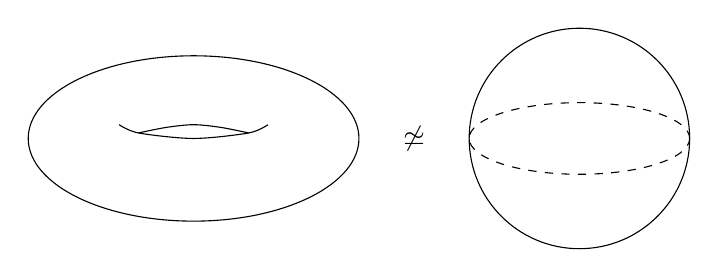
\begin{tikzpicture}[scale=0.35]
        \draw (0,0) ellipse (6 and 3);
        \draw plot [smooth] coordinates{(2.7,0.5) (2, 0.2) (0,0) (-2, 0.2) (-2.7, 0.5)};
        \draw plot [smooth] coordinates{(2, 0.2) (1, 0.4) (0, 0.5) (-1, 0.4) (-2, 0.2)};
        \draw (14,0) circle (4);
        \draw[dashed] (14,0) ellipse (4 and 1.3);
        \node at (8,0) {$\not\simeq$};
      \end{tikzpicture}
    \end{center}
  \end{example}

  Furthermore, like homeomorphisms, homotopy equivalence is a relation on the set of all topological spaces. 
  \begin{enumerate}
    \item Identity. Just set $f, g = id_X$
    \item Symmetricity. Given $X \simeq Y$ with $f: X \longrightarrow Y, g: Y \longrightarrow X$, we set $f^\prime \equiv g$ and $g^\prime \equiv f$ and use these functions $f^\prime, g^\prime$ to find out that $Y \simeq X$. 
    \item Transitivity. Let us have $X \simeq Y$ with functions $f_1, g_1$ and $Y \simeq Z$ with functions $f_2, g_2$. Then, we define new functions 
      \begin{equation}
        f_3 \equiv f_2 \circ f_1: X \longrightarrow Z, \; g_3 \equiv g_1 \circ g_2: Z \longrightarrow X
      \end{equation}
      which follows to $f_3 \circ g_3 = id_Z$ and $g_3 \circ f_3 = id_X$. 
  \end{enumerate}

  \begin{theorem}
    $\mathbb{R}^n$ is homotopically equivalent to a point $\{0\}$.
  \end{theorem}
  \begin{proof}
    We claim that the continuous maps (canonical injection and projection)
    \begin{equation}
      id_{\mathbb{R}^n}: \{0\} \longrightarrow \mathbb{R}^n , \; p_0 : \mathbb{R}^n \longrightarrow \{0\}
    \end{equation}
    have the property that 
    \begin{equation}
      id_{\mathbb{R}^n} \circ p_0 \simeq id_{\mathbb{R}^n} , \; p_0 \circ id_{\mathbb{R}^n} \simeq id_{\{0\}}
    \end{equation}
    The right-hand homotopy is trivial since $id_{\mathbb{R}^n} \circ p_0 = id_{\mathbb{R}^n}$, and as for the left-hand homotopy, we can explicitly define it as
    \begin{equation}
      H: [0,1] \times \mathbb{R}^n \longrightarrow \mathbb{R}^n
    \end{equation}
    with
    \begin{equation}
      H(t, x) \equiv (t) (id_{\mathbb{R}^n} \circ p_0 )(x) + (1-t) \, id_{\mathbb{R}^n} (x) = (1-t)\, id_{\mathbb{R}^n} (x)
    \end{equation}
  \end{proof}

  \begin{example}
    $S^1 \simeq \mathbb{R}^2 \setminus \{0\}$, and more generally, $S^{n-1} \simeq \mathbb{R}^n \setminus \{0\}$. We can see this with the canonical injection and projections
    \begin{equation}
      id_{\mathbb{R}^2}: S^1 \longrightarrow \mathbb{R}^2 \setminus \{0\}, \; \pi_{S^1}: \mathbb{R}^2 \setminus \{0\} \longrightarrow S^1
    \end{equation}
    and find that
    \begin{equation}
      id_{\mathbb{R}^2} \circ \pi_{S^1} \simeq id_{\mathbb{R}^2}, \; \pi_{S^1} \circ id_{\mathbb{R}^2} \simeq id_{S^1}
    \end{equation}
    where the right-hand homotopy is trivial, and the left hand homotopy is defined explicitly as
    \begin{equation}
      H(x, t) \equiv t (id_{\mathbb{R}^2} \circ \pi_{S^1})(x) + (1-t) (id_{\mathbb{R}^2})(x)
    \end{equation}
  \end{example}

  \begin{example}
    A map $f: S^1 \longrightarrow X$ is null homotopic precisely when it can be continuously extended to a map 
    \begin{equation}
      \Tilde{f}: D^2 \longrightarrow X
    \end{equation}
    that agrees with $f$ on the boundary $\partial D^2 = S^1$. Visually, the existence of $\Tilde{f}$ allows us to continuously deform the image of $f$ in $S^1 \oplus X$ to a level curve $f(x) = c$ existing in $S^1 \oplus X$. 
  \end{example}

  \begin{theorem}
    A space $X$ is contractible if any only if the identity map from $X$ to itself, which is always a homotopy equivalence, is null homotopic. 
  \end{theorem}

  \begin{example}
    Let $Y$ be the following gray subset of the plane, and let $X$ be the figure-8 shape. 
    \begin{center}
      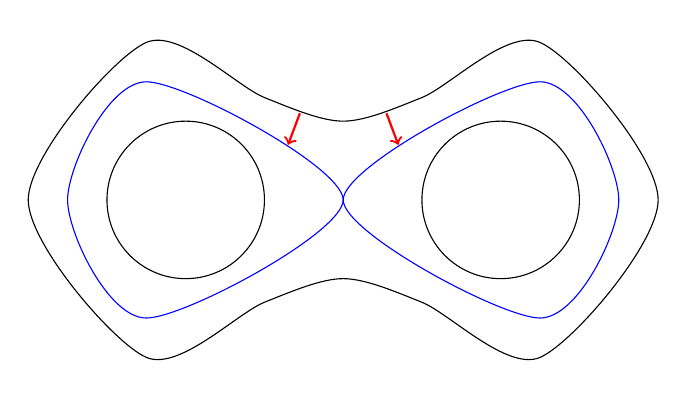
\begin{tikzpicture}
        \draw (-2,0) circle (1);
        \draw (2,0) circle (1);
        \draw[blue] plot [smooth cycle] coordinates{(0,0) (-2.5, 1.5) (-3.5, 0) (-2.5, -1.5)};
        \draw[blue] plot [smooth cycle] coordinates{(0,0) (2.5, 1.5) (3.5, 0) (2.5, -1.5)};
        \draw plot [smooth cycle] coordinates{(0, 1) (1,1.3) (2.5, 2) (4,0) (2.5, -2) (1, -1.3) (0, -1) (-1, -1.3) (-2.5, -2) (-4, 0) (-2.5, 2) (-1, 1.3)};
        \draw[thick, red, ->] (0.55, 1.1)--(0.7,0.7);
        \draw[thick, red, ->] (-0.55, 1.1)--(-0.7,0.7);
      \end{tikzpicture}
    \end{center}
    Then $Y \simeq X$, where the corresponding functions are
    \begin{align}
      & F: X \longrightarrow Y, \text{ the canonical inclusion} \\
      & F: Y \longrightarrow X, \text{ the projection onto X}
    \end{align}
    Then, $G \circ F = id$ and $F \circ G$ is homotopic to the identity, with homotopy defined
    \begin{equation}
      H(x, t) \equiv t (F \circ G) (x) + (1-t) (id_Y) (x)
    \end{equation}
    which can be visualized by $H(x, s)$ being the point you get from $x$ by moving a fraction $s$ along the red arrow towards $X$. 
  \end{example}

